\section{Analytical design examples}
\label{sec:engineering}
The examples in this section are exact models, not simulations. All thresholds, probabilities and optimization values are derived below or in \cref{app:worked}. The accompanying plots display the formulas and geometry. They do not supply a numerical premise for a proof.

\subsection{Three assets and an obstruction to two-domain protection}
Place contacts at $(-1,0)$, $(1,0)$ and $(0,3/2)$ with common radius $6/5$. Around the three pairwise midpoints $(0,0)$, $(-1/2,3/4)$ and $(1/2,3/4)$, take triangular target patches with offsets
\[
(-1/20,-1/20),\quad(1/20,-1/20),\quad(0,1/20).
\]
Each patch lies in exactly its intended pair of disks; the complete inequalities are given in \cref{app:worked}. Thus
\[
\mathcal A_T=\{\{1,2\},\{1,3\},\{2,3\}\}.
\]
Two contacts always cover every target point, but two domains cannot protect all three patches against a domain loss. If the first two contacts have different colors, the third must differ from both to avoid a monochromatic pair. Three domains are necessary and sufficient. This elementary odd-cycle argument distinguishes overlap count from a decomposition into independently surviving layers.\footnote{The example is a finite illustration of cover-decomposition and polychromatic-coloring questions, which have a substantial prior literature~\cite{polychromatic}. It is not presented as a newly discovered coloring obstruction.}

\begin{figure}[!htbp]
\centering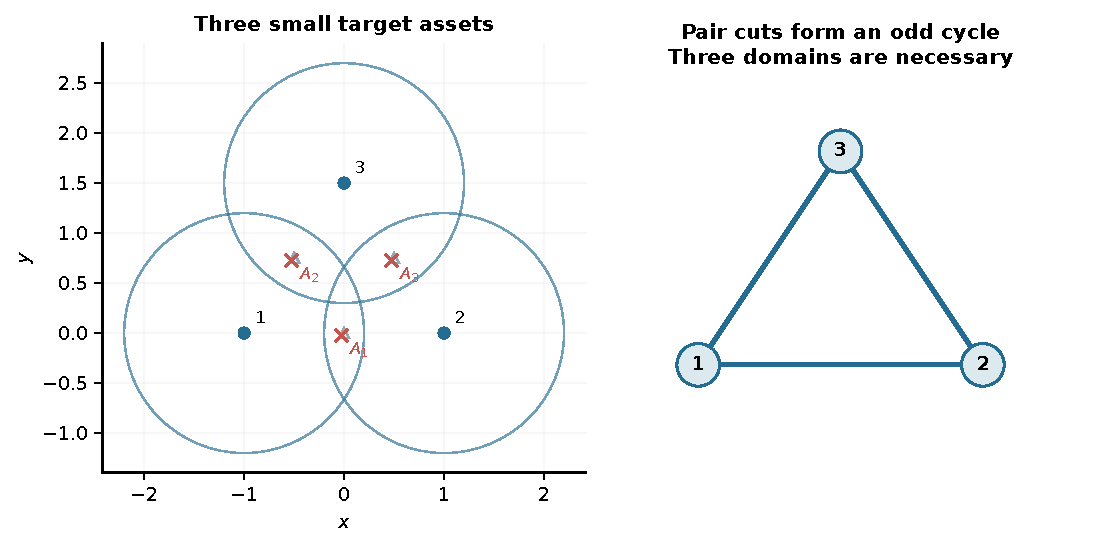
\includegraphics[width=\textwidth]{figures/odd-cycle.pdf}
\caption{The three exact target patches and their critical pair cuts. Each patch can be checked by the rational squared-distance inequalities in the appendix. The cut graph is an odd cycle.}
\end{figure}

Under unit total protection resource and unit protection coefficients, the cut cost is
\[
\kappa_T(c)=\min(c_1+c_2,c_1+c_3,c_2+c_3).
\]
If the full resource is used, this equals $1-\max_i c_i\le2/3$. Equality holds at $c_i=1/3$. Equivalently, a uniform dual distribution on the three cuts gives $\mu=2/3$, proving the exact optimality value through \cref{thm:protection}. For independent contact failure probability $p$, the target survives precisely when at most one contact fails, giving $1-3p^2+2p^3$.
\FloatBarrier

\subsection{A square target with four corner contacts}
Take target $[-a,a]^2$ with $a=3/5$, sites $(\pm1,\pm1)$ and nominal radius $9/5$. Label them in order as $(-1,-1)$, $(-1,1)$, $(1,-1)$ and $(1,1)$. The critical patterns are
\begin{equation}\label{eq:panel-cuts}
\{1,2\},\quad\{1,3\},\quad\{2,4\},\quad\{3,4\}.
\end{equation}
To verify completeness, write $u=\max(|x|,|y|)$ and $v=\min(|x|,|y|)$. The second-nearest squared distance is
\[
2+u^2+v^2-2u+2v,\qquad 0\le v\le u\le a.
\]
This convex quadratic has maximum $2+2a^2=68/25$ at a vertex of the parameter triangle. The two nearest corners share a side; at a tie the active set contains one of those adjacent pairs. Since $81/25>68/25$, every active set contains a listed pair.

The point $(-11/20,0)$ has squared distances $481/400$ to the left corners and $1361/400$ to the right corners. Since $(9/5)^2=1296/400$, its active set is exactly $\{1,2\}$. The three symmetric points realize the other pairs. This proves \cref{eq:panel-cuts} without an enumeration procedure.

\subsection{An exact power--resilience staircase}
For the same geometry, let $t=r^2$ and assign unit deletion costs. The maxima of the first through fourth ordered squared distances are
\[
2,\qquad68/25,\qquad89/25,\qquad128/25.
\]
The formulas for all four distances and their maxima are derived in \cref{app:worked}. Therefore the complete deletion-cost frontier is
\begin{equation}\label{eq:panel-staircase}
K_T(t,\mathbf1)=
\begin{cases}
0,&t<2,\\
1,&2\le t<68/25,\\
2,&68/25\le t<89/25,\\
3,&89/25\le t<128/25,\\
4,&t\ge128/25.
\end{cases}
\end{equation}
Closed disks accept every left endpoint. For tolerance of $q$ arbitrary unit-cost deletions, the required frontier height is at least $q+1$. A request to tolerate two losses thus requires $t\ge89/25$, whereas nominal $t=81/25$ tolerates only one.

\begin{figure}[!htbp]
\centering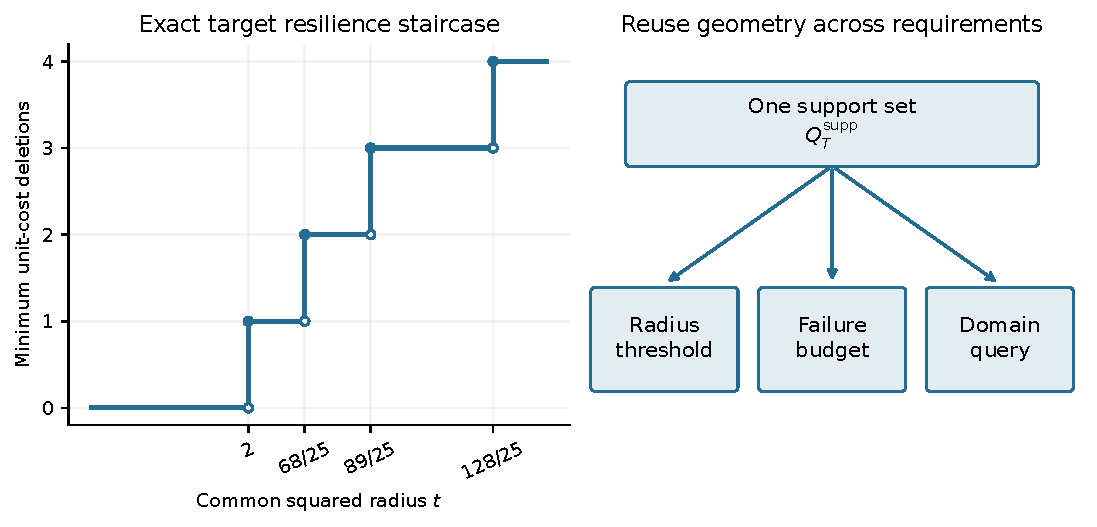
\includegraphics[width=\textwidth]{figures/analytical-frontier.pdf}
\caption{The exact step function in \cref{eq:panel-staircase}. Filled markers indicate accepted equality at each power threshold. The right-hand schematic shows how one support set answers radius, budget and domain queries.}
\end{figure}

\subsection{The resource optimum and the role of duplication}
Each contact occurs in exactly two of the four critical pairs. Under $\sum_i c_i\le1$,
\[
\sum_{A\in\mathcal A_T}c(A)=2\sum_i c_i\le2.
\]
At least one pair therefore has cost at most $1/2$. Uniform allocation $c_i=1/4$ gives cost $1/2$ for every pair. It is optimal, and the uniform distribution on the four cuts is a dual certificate.

Two coincident copies at every corner raise the minimum number of individual unit-cost deletions from two to four. Yet under one fixed linear protection budget, the optimal value stays $1/2$ by \cref{prop:duplication}. No contradiction arises: the unweighted count assumes one cost per copy, whereas the protection problem optimizes total allocated cost under a fixed resource constraint.

Adding a fifth contact at the origin with the same radius $9/5$ gives another distinction. Its disk alone covers the target because $x^2+y^2\le18/25<81/25$. Allocate the full protection budget to that contact to obtain guaranteed deletion cost one. No cut can cost more than the total allocation one, so this is optimal. The bound follows analytically without identifying every new target cut.

\subsection{Wiring and reliability}
Assign the columns to two domains. The left-pair witness depends only on the left domain, and the right-pair witness depends only on the right domain. Both must remain functioning for full target coverage. Assigning the diagonals instead puts one member of every critical pair in each domain, so either domain alone covers the target.

Thus one-domain-loss tolerance fails for column wiring and holds for diagonal wiring. Under independent domain failure probability $p$, reliability is $(1-p)^2$ and $1-p^2$, respectively. The values at $p=1/10$ are $81/100$ and $99/100$. These are exact probabilities in the stated two-domain model. An implementation must justify its domain failure law before interpreting them as hardware reliability.

The exact squared sensing thresholds are $89/25$ for column wiring and $68/25$ for diagonal wiring. Their symbolic derivation in \cref{app:worked} also gives the worst target locations. The nominal $81/25$ lies strictly between them, so the wiring difference changes the accepted design without moving or adding a sensor.

\subsection{Exact uncertainty allowances}
Independent center errors in Euclidean balls of radius $\epsilon$ erode the effective radius to $9/5-\epsilon$ by \cref{cor:erosion}. Two-contact target coverage is therefore robust exactly when
\begin{equation}\label{eq:panel-error}
\epsilon\le\frac{9-\sqrt{68}}5.
\end{equation}
For independent displacement boxes of halfwidth $1/10$, the exact critical squared radius is $157/50$, derived in \cref{app:worked}. Since $157/50<81/25$, the nominal design meets that box-error requirement. The box formula and ball formula are different exact uncertainty supports, not interchangeable numerical tolerances.

\subsection{A three-dimensional sharpness example}
Let the four sites be the vertices
\[
(1,1,1),\quad(1,-1,-1),\quad(-1,1,-1),\quad(-1,-1,1)
\]
of a regular tetrahedron, and let the target be its convex hull. Each site has squared norm three and their centroid is zero. If $x=\sum_i\lambda_i c_i$ is a convex combination of the vertices, then
\begin{equation}\label{eq:tetra-variance}
\sum_i\lambda_i\|x-c_i\|^2=3-\|x\|^2.
\end{equation}
At least one vertex distance squared is therefore at most $3-\|x\|^2$. Away from zero this is strictly less than three. At zero all four distances equal $\sqrt3$. Thus ordinary one-contact coverage has exact radius $\sqrt3$ and its unique worst location is the interior point zero.

All four sites tie there with rank three. No pair or triple of these vertices alone determines the unique three-dimensional equal-distance location. The example shows why the general support theorem allows $d+1$ sites on a $d$-dimensional target. More generally, the same variance identity applies to a cospherical simplex whose center lies in its interior.\footnote{The example shows that the support-size bound cannot generally be reduced from $d+1$ to $d$ by restricting to lower-order equal-distance systems. It is not a lower bound against arbitrary encodings of the target.}

\begin{figure}[!htbp]
\centering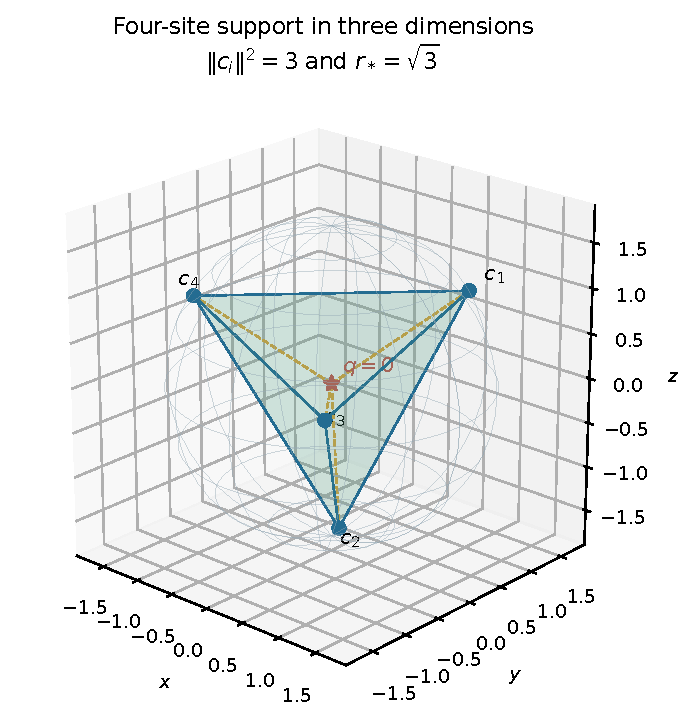
\includegraphics[width=.75\textwidth]{figures/tetrahedron-support.pdf}
\caption{The three-dimensional support example. The tetrahedron, its four sites, the common sphere and the unique worst point illustrate \cref{eq:tetra-variance}. The exact proof is the barycentric identity, not a sampled surface or numerical optimization.}
\end{figure}
\FloatBarrier
